\chapter[MC event generation]{Understanding theory predictions via Monte-Carlo event generation}
\label{chap:MC}

Although we have nowadays a very elegant and complete theoretical description of particle physics, is not always evident how to translate this theory in actual predictions, to compare with measurements. Moreover, on the case of hadronic colliders, as the LHC, it's even more difficult due to the particularities of strong interaction. On this subject, a set of tools and approaches have been developed in order to be able to make accurate predictions from theory that could be directly researched for on the experiments, as CMS or ATLAS for example. In the present chapter, we describe such tools and formalisms and a set of studies comparing the predictions these tools to data. 

\section{Mote-Carlo simulations}
\label{sec:MC}

The Monte-Carlo simulations use random numbers and large samplings to calculate mathematical quantities in complex configurations, as integrals or probabilities. The typical example is on how to calculate the integral of a one-dimensional function. One can throw several random coordinates pair in the Cartesian plane and count how many of them are under the function. Then the integral of the function will be proportional to the fraction of points under the curve to the total thrown points. Larger the number of points, closer the estimation to the real value. An illustration of the procedure can be seen in figure~\ref{fig:mc_int}.

\begin{figure}[!Hhtbp]
  \begin{center}
    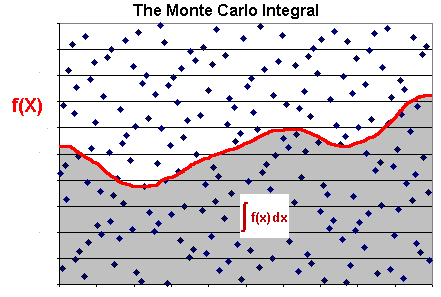
\includegraphics[width=0.6\textwidth]{figs/mc_integral.png}
    \caption{Integration using Monte-Carlo methods}
    \label{fig:mc_int}
  \end{center}
\end{figure}

A similar method is used to simulate proton-proton collisions. This simulation is used to generate ``random'' events and to calculate quantities, as the cross section, for a given physical process. Each event represent the final state of a collision, i.e. the set of particles produced from the collision and seen by a detector. Such simulations comprehend different stages: first, the partonic processes making reference to the interaction between the partons inside the proton; second, the hadronization of the particles produce from parton interactions; and third, the simulation of the interaction between the hadrons (from second step) and the detector material. Such events are used to evaluate predictions from theory in the frame of a specific experiment. Whereas the hadronization and detector simulation are well-known physical processes, new theories predictions rely basically on the partonic level, where the fundamental interaction processes take part.

\subsection{Parton simulation}
\label{sec:parton}

The parton model was initially proposed by Richard Feynman in 1969, as a method to understand collisions of non-fundamental particles. The model consider a non-fundamental particle, as a proton or a neutron, composed of a given number of point-like fundamental particles. When a collision occur the point-like particles inside have a major probability to scatter. For example, when an electron is fired against a proton the most of the interactions will between the electron and the fundamental components of the proton, $u$ and $d$ quarks. This ``hard'' components are called \textit{valence} quarks. Surrounding them there are the \textit{sea} quarks and gluons.

However, as the energy of the collision increases the probability to scatter a sea component, quark or gluon, increases. In addition, even if the valence quarks of a proton are the $u$ and $d$ quarks, heavier quarks can appear in the sea, as the $b$, $c$ or $s$ quarks. The probability to interact with a component, valence or sea, is described by parton distribution function, commonly called PDF. A PDF $f\equiv f(x,Q^{2})$ represent the number density of a given quark or gluon as a function of the energy scale $Q^{2}$ and the fraction of momentum carried by the parton $x$. In figure 

\begin{figure}[!Hhtbp]
  \begin{center}
    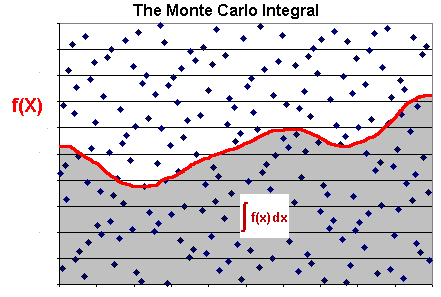
\includegraphics[width=0.6\textwidth]{figs/mc_integral.png}
    \caption{Integration using Monte-Carlo methods}
    \label{fig:mc_int}
  \end{center}
\end{figure}

\subsection{Hadron simulation}
\label{sec:hadron}

\subsection{Detector simulation}
\label{sec:detector}


\section{Tools}
\label{sec:tools}

\subsection{Matrix-element generators}
\label{sec:ME}

\subsection{Hadron generators}
\label{sec:Had}

\subsection{Detector simulation}
\label{sec:det}

\section{Validation on data}
\label{sec:val}

